\documentclass[12pt]{scrartcl}
\usepackage{geometry}                % See geometry.pdf to learn the layout options. There are lots.
\geometry{a4paper}                   % ... or a4paper or a5paper or ... 
%\geometry{landscape}                % Activate for for rotated page geometry
%\usepackage[parfill]{parskip}    % Activate to begin paragraphs with an empty line rather than an indent
\usepackage{graphicx}
\usepackage{amssymb}
\usepackage{epstopdf}
\DeclareGraphicsRule{.tif}{png}{.png}{`convert #1 `dirname #1`/`basename #1 .tif`.png}
%\usepackage{}
\usepackage{color}
\definecolor{Orange}{rgb}{1,0.5,0}
\definecolor{HBGreen}{rgb}{0,0.8,0}
\newcommand{\todo}[1]{\textsf{\textbf{\textcolor{Orange}{[Todo: #1]}}}}
% Macro for writing in the margin comments on what is left to be done.
\newif\ifdraft
               \drafttrue
               %\draftfalse
\ifdraft
\newcounter{ournotecounter}
\newcommand{\ournote}[1]{%
\textsf{\textbf{\textcolor{Orange}{[#1]}}}}
\newcommand{\alnote}[1]{%
\textsf{\textbf{\textcolor{HBGreen}{[#1]}}}}
\typeout{Compiling in draft mode.}
\else
\newcommand{\ournote}[1]{}
\newcommand{\bigournote}[1]{}
\typeout{Compiling in final mode.}
\fi

\title{Modelling Emission of Climate gases }
\subtitle{Using mobile sensing data}
\author{Anders Lehmann}
\date{July 2014}                                           % Activate to display a given date or no date

\begin{document}
\maketitle
\newpage
\pagenumbering{roman}
\tableofcontents
\newpage	
\pagenumbering{arabic}	
%\section{}
%\subsection{}
\section{Introduction}

The proliferation of smartphones brings new opportunities to researchers who are studying the behaviour of modern human beings. For research in mobility and transport the proliferation of smartphones yields the potential to lower the cost for gathering relevant data to near zero \cite{Liu2013}.
In this project, smartphones are a central requisite as an tool information and data gathering tool. The main idea in the project is to gather from real life activities, create models to interpret the data, and visualisations from the output of the models. 

In modern societies, carbon emissions from transport are a large and growing part of the total carbon emissions from human activities. For instance, in Denmark the emission of carbon dioxide from transport was 24 \% of the total Carbon emissions in 2012 \cite{nielsen2014}, and road transport is responsible for 67 \% of the Carbon emissions from transport. In order to be able to create viable measures to lower the carbon emissions from passenger transport, there is a need for more detailed models quantifying these emissions. By using data from smartphones we aim to obtain more accurate information on where and when emissions from transport are created. These models can help policy makers and planners make informed decisions on future changes to the road transport system and related infrastructure.

As Carbon emissions are closely related to the fuel consumption, experiments were designed and carried out which gathered from an onboard smartphone  driving-related data and data on the amount of fuel consumed.

\todo{can be ommited?:}
To accurately model Carbon emissions from smartphone data, an experiment was performed in order to establish a ground truth\todo{ground truth: explain what and why?}. 

We chose to use some old car \todo{exact details? btw, use different cars for a broader range of experiments?} for the experiments and thus 
\todo{this sounds like a poor choice and excuse? Can we say that we aim for getting data also from all includung old cars? Btw, what about the instrumenting software that you had trouble with but which our developers now have instrumented on our department car? Would that make that your statement above obsolete?} had to create an accurate fuel consumption measuring method, which did not involve instrumenting the vehicles. 


The remained of the paper is organized as follows:
In Section \ref{sec:relwork} we review related work, including methods for measuring the fuel consumption and for creating related models of fuel consumption from sensor data  Additinoally, we briefly review methods to determine different driving styles and driving modes.
In Section \ref{sec:modeling} the models used to convert the experimental data into emission data are presented. 
The results of the experiments which partly relate to fuel consumption measurement and modeling and partly to reliable detection of driving modes, are presented in Section \ref{sec:results} and the paper is concluded in Section \label{sec:conclusions}.
\section{Climate change policy development}\label{politics}
\subsection{Climate change organisations}
It has been decided in the United Nations to create two bodies for devising policies for managing the anthropogenic global warming. The main political body is the United Nation Framework Convention for Climate Change (UNFCCC) \cite{schipper2009}. The name refers to both a convention created in 1994, and a secretariat that services the operation of the Convention. This body is tasked with creating policy initiatives and negotiate treaties with the members of the UN. A visible part of these negotiations are the COP (Conference of parties) meetings held annually. Since 154 nations have ratified the convention, the negotiations are very difficult, and progress in for instance agreeing on firm goals and plans to reach the goals is slow \cite{pielke1998}.

To support the UNFCCC with scientific knowledge the Intergovernmental Panel on Climate Change (IPCC) was created. The panel gathers scientific evidence into reports on different aspects of climate change, the root causes, the consequences and ways to mitigate and adapt.

Even though the panel is a scientific panel, it is also a part of a political process. This means that the reports made by IPCC, especially the "summary for policy makers" are also heavily negotiated by the participating government officials.

The latest reports from IPCC are the AR-5 (fifth assessment report) series .

The IPCC reports are divided into sections, done by different workgroups. Workgroup 1 delivers a scientific background section containing the latest scientific knowledge about emissions, measured consequences, melting of Icecaps etc. As a new feature in the assessment report a number of scenarios are envisioned, to estimate the consequences of different policies. The scenarios are called "Representative Concentration Pathways", and are named by the expected rise in global mean temperature. Four scenarios are envisioned in the report: RCP2.5, RCP4.5, RCP6, RCP8,5 \cite{stocker2013climate}. These scenarios are then used as a guiding principle for the rest of the sections in the AR-5.

The workgroup 1 report is generally viewed as a high quality and reliable source of knowledge.

Workgroup 2 delivers a report on "Impacts, Adaptation and Vulneralbility". 

Workgroup 3 is about mitigation of climate change.



\subsection{Climate change mitigation}From the start of the debate about how to combat Anthropogenic Global Warming, there have been two competing approaches. The mitigation approach, where an effort is made for reducing the emissions of climate gases, is the approach which has received the most attention\cite{Pielke2007}. The EcoSense project is part of the mindset behind this approach. Whereas the mitigation approach previously has focused on creating more efficient machines, to either produce energy with less emissions or produce machines that produce more useful work per energy unit\cite{Chakraborty2013}, EcoSense focuses on how the machines are used in combination. So instead of focusing on a single energy consuming item, we are trying to analyse how the energy consumption changes as the individual items work together. In other words we are developing tools for studying network effects in the transportation sector, as well as in other sectors.


\subsection{Climate change adaptation}
The second approach is called the Adaptation approach. Since it is probable that there will be significant changes in the climate, even if we succeed in keeping the $CO_2$ emissions within the agreed limits, we have to invent ways to adapt to these changes. The Adaptation approach has not received much attention or research funding, but projects like EcoSense will also have an impact in determining how to adapt to changes in weather patterns. It seems that IPCC in the fifth report from Working Group 2 is beginning to give more attention the Adaptation approach, as a consequence of realising that some level of Climate Change is inevitable \cite{kelly2000}\cite{smithers1997}.


\section{$CO_2$ Modelling}\label{modelling}

In this section the IPCC methodology for calculation of emission of climate forcing gases from transportation will be described. The focus of the IPCC approach is to offer methods for building national inventories for climate gas emissions.

\subsection{IPCC methodology}
The IPCC has made a number of reports on how to calculate emissions of climate forcing gases and pollutants. The gases that IPCC is describing methods for are divided into four groups: 

Group 1 are pollutants where a detailed methodology for estimating the emission from activity data, such as driving conditions, and engine conditions.
\begin{table}[!ht]
  \centering
  \begin{tabular}{@{} | l|c |@{}}
    %\toprule
    %Specie & abbreviation \\ 
    %\midrule
\hline
 \multicolumn{2}{| l |}{Group 1}   \\
\hline
Carbon monoxide & CO\\ 
Nitrogen oxides & (NOx: NO and NO2)\\
Volatile organic compounds &(VOCs)\\
Methane &(CH4)\\
Non-methane VOCs &(NMVOCs)\\
Nitrous oxide &(N2O)\\
Ammonia &(NH3)\\
Particulate matter &(PM)\\
\hline
 \multicolumn{2}{| l |}{Group 2 }\\
\hline
Carbon dioxide & (CO2) \\
Sulphur dioxide & (SO2) \\
Lead & (Pb)\\
Arsenic & (As)\\ 
Cadmium & (Cd)\\ 
Chromium & (Cr) \\
Copper & (Cu)\\
Mercury & (Hg) \\
Nickel & (Ni) \\
Selenium & (Se)\\ 
Zinc & (Zn)\\
\hline
 \multicolumn{2}{| l |}{Group 3} \\
\hline
Polycyclic aromatic hydrocarbons & (PAHs) \\
Persistent organic pollutants & (POPs)\\
Polychlorinated dibenzo dioxins & (PCCDs)\\
Polychlorinated dibenzo furans &  (PCDFs)\\
\hline
 \multicolumn{2}{| l |}{Group 4}\\
\hline
Alkanes & (CnH2n+2)\\
Alkenes &(CnH2n)\\
Alkynes & (CnH2n-2)\\
Aldehydes & (CnH2nO)\\
Ketones & (CnH2nO)\\
Cycloalkanes & (CnH2n)\\
Aromatic compounds& -\\
\hline
  %  \bottomrule
  \end{tabular}
  \caption{IPCC considered species}
  \label{tab:group1}
\end{table}


Group 2 are pollutants which can be estimated from fuel consumption, when there is a direct connection between the burning of fuel and the emission. 
The precision of the estimates of emissions of the Group 2 pollutants are regarded as good as the precision of the estimations for the Group 1 pollutants, even if the methodology differs.
Group 3 and Group for pollutants are organic compounds, where no detailed methodology exist for estimating the emission, so a simple method is used to calculate the emission.

The fourth group of pollutants are species, where the emission is calculated as a fraction of the Non Methane Volatile Organic Compound (NMVOC).
  
When considering Climate forcing gases the most important gases are in Group 1 and 2, thus this is what the focus has been on in this phd study, the most important being $CO_2$, $CH_4$ and $NO_2$.

The way emission inventories are created are described in the the Guidelines from IPCC . In the guidelines three different methods are described, each method more accurate than the previous \cite{Ntziachristos2012}. 

\subsubsection{IPCC Tier 1 model} 

The Tier 1 method is based on numbers for national sales of hydrocarbons (Gasoline, Diesel, Natural gas etc.). These numbers are readily available for most countries and are converted into emission inventories by multiplying emissions factors (grams of the specie pr kilogram of fuel) for each type of fuel. The Tier 1 method is the simplest, but also most crude way of estimating the national emissions, as it does not account for import or export of fuel, and that not all emissions are directly related to fuel consumption. The only data points needed are: Volume of sales of the different fuel types and the emission factors for the different fuel types.

\begin{equation}
	E^{CALC}_p = \sum_i{V_{sales,i}*e_{i,p}}
\end{equation}

Here the $E^{CALC}_p$ is the calculated emission, where $i$ is the fuel type,$V_{sales,i}$ is the sales for fuel type $i$ and $e_i$ is the emission factor for the fuel type. $p$ is the pollutant, for which we are finding the emission.

\subsubsection{IPCC Tier 2 model} \alnote{ Size of data (large)}
In the Tier 2 method the emission inventories are estimated by estimating the traffic volumes for different categories of vehicles, and multiplying emission factors (gram pr kilometre) for each category. The vehicles are divided into six main categories: Passenger Car, Light Duty vehicles, Heavy Duty vehicles, Buses, Mopeds and Motorcycles. For each of the main categories, a subdivision is made, to accommodate for different emission characteristics stemming from pollution regulation, fuel type and engine size. For instance, in Europe, passenger gasoline cars are subdivided into 13 different types, according to the legislation governing allowed emissions. These regulations has been changed and tightened 13 times since the first emission control legislation was ratified in the early nineties. For each vehicle category and vehicle type and legislation class, activity data has to be obtained. The activity data consist of the number of vehicles, and the number of kilometres they drive pr year, for each class. The IPCC has generated tables of emission factors (as g/km) for each class of vehicles. By multiplying these emission factors with the estimated kilometres and number of vehicles in the class, the total emission of a pollutant can be estimated for the vehicle class. The total annual emission from transport can then be calculated as the sum of all the vehicle classes.

\begin{equation}
	E^{CALC}_p = \sum_v\sum_i{D_{v,i}*e_{i,v,p}}
\end{equation}

Here the $E^{CALC}_p$ is the calculated emission, where $i$ is the fuel type,$D_{v,i}$ is the estimated distance travelled vehicle type v and fuel type $i$ and $e_{i,v,p}$ is the emission factor for the fuel type. $p$ is the pollutant, for which we are finding the emission.

\subsubsection{IPCC Tier 3 model} 
The Tier 3 method takes the Tier 2 methods and improve on the estimated emission, by also considering the velocity distribution of the travelled distances, and by considering the effects of cold-starts and vehicle age on the total emissions.

There are two ways proposed to calculate the effects of speed on exhaust emissions. Either by dividing the travelled distance into road types with different speed characteristics, i.e. urban, rural and highway. In this case the total emission for a vehicle class will be calculated as the sum of the product of travelled distance on a road type and the emission factor for that road type and vehicle type.
\begin{figure}[!ht]
\begin{center}
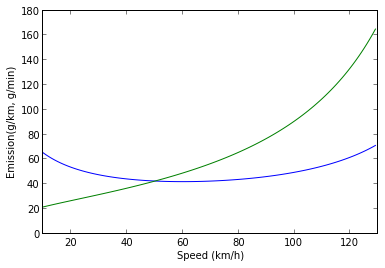
\includegraphics{emission_vs_speed.png}
\caption{{\bf Emission factor as a function of speed. 
g/km blue. g/min green}}
\label{emission_vs_speed}
\end{center}
\end{figure}

The other method uses a measured speed to emission curve and a speed distribution function to estimate the emission. For some pollutants an emission factor function is given, but for pollutants that are directly linked to fuel consumption (i.e. $CO_2$) a fuel consumption function of speed is given. For $CO_2$ the relationship between emission an fuel consumption is given by the formula \ref{emission_from_fc}.

\begin{equation}\label{emission_from_fc}
E^{CALC}_{co_2}, km = 44,011*\frac{ FC^{CALC}}{12,011 + 1,008 *r_{H:C} + 16,000 * r_{O:C}}
\end{equation}

This formula is based on the assumption that all fuel is consumed, i.e. that each carbon atom in the fuel is oxidised into $CO_2$, which have the molar weight of $44,001$. The numerator $FC^{CALC}$ is the calculated fuel consumption factor, and this is divided with the molar weight of carbon plus the molar weight of hydrogen multiplied with the ratio of hydrogen to carbon ,$r_{H:C}$, plus the molar weight of oxygen multiplied with the ratio of oxygen to carbon, $r_{O:C}$,in the fuel. There are tables for different ratios $r_{H:C}$ and $r_{O:C}$ for different fuel types, given in the COPERT IV methodology guidebook \cite{Ntziachristos2012}.

As an example, passenger vehicles that are regulated by EURO 1 the fuel consumption factor curve is given by equation� \ref{speed}. The coefficients $a$ to $e$ are given for the different engine sizes and pollution regulations. 


\begin{equation}\label{speed}
FC = \frac{a + c*V + e*V^2}{1 + b*V + d*V^2}
\end{equation}
An emission factor (in g/km) versus speed curve can be seen in figure \ref{emission_vs_speed} for a vehicle with engine size less than $1,4 l$  \cite{Mellios2011}, as the blue curve. From the curve it can be seen that the emission factor is larger for low speeds and for high speeds an lowest at moderate speeds (app. 60 km/h). The higher emission factor for low speeds is higher because the power of the engine is underused and therefore not very many kilometres are gained. For higher speeds the opposing forces from wind and friction in bearing, force the engine to work harder, and therefore has a higher emission factor. If instead we look at the emission pr minute, by multiplying the emission curve with the speed, we get the green curve. From the green curve it can be seen that the emission pr time unit is a monotonic growing function, which resembles a second order polynomial. The force of the wind on an object is proportional to the square of the speed.

 The emission is calculated as the integral of the speed distribution multiplied by the emission function as seen in equation \ref{integral}.

\begin{equation}\label{integral}
e_{i,k,r} = \int{e(V)*f_{k,r}(V)dv}
\end{equation}

($i$ is the the pollutant for which the emission is calculated).

The data needed to use the Tier 3 method is quite extensive. For each of the 13 vehicle classes (divided by fuel type, vehicle size) activity data for milage for urban, rural and highway travel, hot start/cold start, as well as data for the number of vehicles in each emission regulation is needed. Fortunately the program COPERT 4 contains the emission factors, and country specific activity data can be downloaded to use for evaluating national inventories.


\subsection{Modelling emissions from electric vehicles}
The emissions for electric cars are calculated from near real time emission data from Energinet.dk, under the assumption that electric cars will be charged with electricity from the public grid. There is for now no way to detect if the charging of electric vehicles are not done through the public electric grid.

\section{Air pollution dispersion Modelling}
This section gives an overview of different ways for calculation of how the concentration of pollutants change over time and space. Typically we investigate how pollutants move from a pollution source with wind or through diffusion through the area of interest. The concentrations of the species change partly by dilution (the plume widens), and partly by chemical reactions in the atmosphere. The chemical reactions are dependent on different factors, such as light and temperature. In the section on OSPM the effect of the landscape (here a street canyon) is discussed.

\subsection{Euler method}
The Euler method is also called the box model. The area that we want to investigate is divided into boxes. In at least one box there can should be a source of pollution. The concentration of the pollutants in the box can be calculated as the amount of the species coming into the box (either through the walls of the box, from chemical reactions or from soured located inside the box) minus the amount of the species lost (through the walls, deposition or chemical reactions).

For each time step the concentration of each specie is calculated by solving an ordinary differential equation (ODE) and the calculated concentrations are use to determine the start conditions for the next time step, as well as the boundary conditions for the surrounding boxes.

Examples of box models are Danish Eulerian Hemisphere Model (DEHM), which calculates concentration of 63 different species and 120 chemical reactions in different scales (size of boxes).

\subsection{Lagrange}
In the Lagrange method a parcel of air is considered  

\subsection{Atmospheric chemistry}
An important complicating factor of modelling concentration of pollution is the fact that the different pollutants will undergo change due to chemical reactions

\alnote{Is particulate matter modelled in the above mentioned models?}


\subsection{DASK}
DAnish Solver for chemical Kinetic (DASK) is a chemical compiler and solver. The idea of DASK is to automate the code generation for handling chemical reactions. In DASK you give the chemical reactions and their reaction rates as input, and the program transforms the input into fortran code. The generated Fortran code is called inside the ODE solver, so that it is easy to add new chemistry.

Beside the chemical compiler, there is also an easy way of setting up scenarios for the solver to solve. 
\subsection{OSPM}
The Operational Street Pollution Model is a model for calculation of pollution in urban environments. Due to turbulent wind conditions in urban street canyons the pollutants do not mix well with the surrounding air, there will be a tendency to have the heavier pollutants to concentrate on leeward side of the street canyon. The OSPM model considers the effects of street geometry, wind speed, emission factors and atmospheric chemistry (i.e. the $NO - NO_2 - O_3$ cycle).



\section{Internet of Things}
The vision of Internet of Things is to connect devices, across application, geographic and company boundaries. To accomplish this vision, a common language and framework had to be agreed upon. Tim Berners-Lee started this work by creating the Resource Description framework (RDF) in ????. The definition of have spurred the creation of query languages (SPARQL), semantic frameworks (OWL, SKOS), IDE (Prot\'eg\'e, TopBraid composer) and implementations (SESAME, Virtuoso, Talis, RDFLIB ).

\subsection{Linked Data}

\subsection{Semantic annotated data}
\subsection{Linked Devices}
\subsection{Linked Data as an Enterprise Architecture strategy}


\section{Future Research}\label{futurework}
In this section the planned work for the remainder of the phd study will be discussed. The focus of the section is the planned scientific contributions.

\subsection{Improving estimation of emissions for single trips}
As outlined in section \ref{Modelling}, the current modelling focus is to create and maintain national inventories, which leads to a focus on mean values for emission factors, driving patterns and trip patterns. To be able to provide personalised information on specific transportation behaviour, there is a need to provide more detailed models for the emission of single trips. In this section an outline for possible algorithms for reaching that goal is presented.

One proposal is to divide a trip into four different types of driving : Idle, accelerate, cruise and decelerate. For each type of driving a emission profile can be derived and thus the emission for each type can be determined. To total emission for a trip can then be determined as the sum of the emission for each type.

\subsubsection{Idle emissions}\label{Idle}
Detection of idle situations can be done with combination of GPS data and accelerometer data. The GPS data can be used to estimate the speed of the vehicle, and the accelerometer can be used to measure the engine speed to confirm that we are in idle mode. There are some literature about measuring emissions from idling, but it might be necessary to update with new measurements. A possible source for idle emission data could be the approval data for Danish biannual vehicle inspections, since part of the inspection is a measurement of the contents of the exhaust in idle mode.

\subsubsection{Emissions when accelerating}
The horizontal acceleration can be determined by finding the direction of gravity in respect to the device, through a variety of methods. These methods will have to be evaluated to find a suitable solution for the application at hand.
When the gravity direction has been determined, the horizontal acceleration will be either close to zero, when cruising or idle, or have a significant value due to acceleration, turning or deceleration. It is believed that it will be possible to provide a stable algorithm for detecting horizontal acceleration and distinguish between turning and acceleration.

To model the emission from an accelerating vehicle information, such as engine size and vehicle weight, is needed. This information has to be given as input to the model by the user, or be inferred from the Transportation Mode Detection part of EcoSense.

Another input to the model could be the road grade, since the engine will have to work harder, thus emitting more pollutants, if the vehicle is going uphill. By using the GPS data to get information on the position, the road grade can be gleaned from a digital road network. By fusing the information from these different sources the emission modelling  can be further improved.  

\subsubsection{Emissions when decelerating}
When decelerating, there are a couple of different situations to be ware of. The simplest situation is when the vehicle is braking using the mechanical brake. In this situation the engine will typically be in idle mode and the results from section \ref{Idle} can be reused. If the vehicle incorporate regenerative braking, motor braking or automatic transmission the situation is more complex. The proposal is to first ascertain if deceleration can be detected and then in an first approximation used the results from \ref{Idle}
\subsubsection{Emissions when cruising}
In the study of emission models, models for speed dependency of emissions have been found. These models can be used as is if we can determine that we are moving at a constant speed. These models are described in section \ref{Modelling}. The models are developed for emission modelling programs such as COPERT IV, which was developed as part of the EU project ARTEMIS. The models used in COPERT IV can be used to assign a speed dependent emission factor to specific vehicle types, engine sizes and fuel types.
 
\subsubsection{Papers}
A position paper on the state of the art of modelling emission from mobile sensing is planned.

More specialised papers detailing and evaluating the improvements made in this study is also planned.

\subsection{Correlation of trips}
In order to be able to spot inefficiencies in transportation patterns, a way of group, aggregate and correlate different trips are needed. The grouping of trips could be by persons, time of day, seasonal or geographic. The aggregation could be looking for all trips at specific location in a certain time period. Correlation is useful for finding trips which follow a certain route.

In order to solve these problems efficiently, some heuristics may be useful. If a digital road network is available for the area under consideration, each trip can be converted into a subgraph of the  digital road network, under the assumption that vehicles travels along the roads. By having the trips as a graph instead of a time series of GPS locations, will simplify the task of correlation, thus good and efficient algorithms to convert GPS traces to road network graphs is needed.
%\subsubsection{Methodology}
\subsubsection{Impact}

\subsubsection{Papers}
A paper documenting the approach and detailing the possible benefits in terms of finding opportunities for minimising the emission of pollutants through better route planning. I will attend a course at DTU Transport during the autumn concerning "Route Choice Models", to prepare for this.
\subsection{Field trials}
Among the partners in the EcoSense project are some municipalities. The interest from the municipalities in the EcoSense project are among other, to be test sites for the results coming out of the project. In return the researcher partners get real world data to learn from in future research
\subsubsection{S\o nderborg}
In the municipality of S\o nderborg, there have been a long tradition for doing projects with focus to mitigate the threat of Climate Change through minimising the emission of climate forcing gasses. The task of finding ways of minimising the emission for S\o nderborg, has been put to an organisation called "Project Zero". "Project Zero initiates and run campaigns for raising the awareness of climate gas emissions, as well as measure the effects of these campaigns. "Project Zero" has campaigns that target citizens and other campaigns that target the local industry.

As "Project Zero is a partner in EcoSense, we have the possibility to make mobile applications that underpin or are a part of the campaigns "Project Zero" runs. An interesting experiment could be measure the air pollution at the central bridge over Als-sund, and compare with the danish city canyon model OSPM, and traffic data obtained from mobile sensing.

\subsubsection{Herning}
In Herning a project called "Herning cycler til m\aa nen", Herning bikes to the moon. The goal of the project is to get the citizens of the municipality to bike the distance to the moon. To measure the distance travelled on bike, participants can download an mobile application, developed in the EcoSense project. The app sends data to the EcoSense servers, and we thus get the possibility to look into real world transportation.



\subsubsection{Papers}
It would be reasonable to document the results of this real world (or at least outside the laboratory) trials in a number of papers. Each trial has different goals but share a number of tools.

These papers would be evaluating the approach.
\subsection{Visiting researcher}
During the last 2 years of the study I plan to visit an university, to participate in the research as it is performed there. I plan to have the stay at another research group during the teaching free period in the summer of 2015. I am currently actively looking for suitable research groups in other transportation research, air pollution modelling or geographic data research.

\section{Conclusion}

In this paper we have presented a method for modelling Carbon emission from smartphone data and a method for discerning six different driving modes. The Carbon emission model is quite stable with a standard deviation of 0.02. 

The K-means based method for discerning between driving modes is able to discern between four acceleration modes (forward, brake, left turn, and right turn) and two non-accelerating modes.
\end{document}  
